\documentclass[a4paper,12pt,oneside]{book}

%-------------------------------Start of the Preable------------------------------------------------
\usepackage[english]{babel}
\usepackage{blindtext}
%packagr for hyperlinks
\usepackage{hyperref}
\hypersetup{
    colorlinks=true,
    linkcolor=blue,
    filecolor=magenta,      
    urlcolor=cyan,
}

\urlstyle{same}
%use of package fancy header
\usepackage{fancyhdr}
\setlength\headheight{26pt}
\fancyhf{}
%\rhead{
\includegraphics[width=1cm]{logo}}
\lhead{\rightmark}
\rhead{
\includegraphics[width=1cm]{logo}}
\fancyfoot[RE, RO]{\thepage}
\fancyfoot[CE, CO]{\href{http://www.e-yantra.org}{www.e-yantra.org}}

\pagestyle{fancy}

%use of package for section title formatting
\usepackage{titlesec}
\titleformat{\chapter}
  {\Large\bfseries} % format
  {}                % label
  {0pt}             % sep
  {\huge}           % before-code
 
%use of package tcolorbox for colorful textbox
\usepackage[most]{tcolorbox}
\tcbset{colback=cyan!5!white,colframe=cyan!75!black,halign title = flush center}

\newtcolorbox{mybox}[1]{colback=cyan!5!white,
colframe=cyan!75!black,fonttitle=\bfseries,
title=\textbf{\Large{#1}}}

%use of package marginnote for notes in margin
\usepackage{marginnote}

%use of packgage watermark for pages
%\usepackage{draftwatermark}
%\SetWatermarkText{
\includegraphics{logo}}
\usepackage[scale=2,opacity=0.1,angle=0]{background}
\backgroundsetup{
contents={
\includegraphics{logo}}
}

%use of newcommand for keywords color
\usepackage{xcolor}
\newcommand{\keyword}[1]{\textcolor{red}{\textbf{#1}}}

%package for inserting pictures
\usepackage{graphicx}

%package for highlighting
\usepackage{color,soul}

%new command for table
\newcommand{\head}[1]{\textnormal{\textbf{#1}}}


%----------------------End of the Preamble---------------------------------------


\begin{document}

%---------------------Title Page------------------------------------------------
\begin{titlepage}
\raggedright
{\Large eYSIP2016\\[1cm]}
{\Huge\scshape Exploring Wiced Sense \\[.1in]}
\vfill
\begin{flushright}
{\large Chinmay Patil \\}
{\large Imran Khan \\}
{\large Santosh \\}
{\large Uttam \\}
{\large Duration of Internship: $ 10/06/2016-24/07/2016 $ \\}
\end{flushright}

{\itshape 2016, e-Yantra Publication}
\end{titlepage}
%-------------------------------------------------------------------------------

\chapter[Exploring Wiced Sense]{Exploring Wiced Sense}

\section{Abstract}

\hspace{5mm} With hundreds of new ideas for applications of wireless devices it is critical that developers are provided a platform to quickly test their
concepts and bring them to real use. 
\\ \hspace{5mm} This project aims at exploring different aspects of WICED Sense (SIP Module), in order to start
experimenting with sensor technology which will enable the developers to include physical quantities such as temperature , atmospheric pressure ,humidity ,direction, acceleration, yaw, pitch, roll, etc.
\\ \hspace{5mm}
The aspects include understanding the wiced sense sdk inorder to program the device for user specific application , procedure to acquire the data from the wiced tag , saving the acquired data in a online database so that it can be accessible for distant users for processing , visualization of the sensor data on website , making automation related applicatons and path mapping of firebird V robot on a webpage using the sensor data.
\\ \hspace{5mm}
The ultimate goal of the project is to create a basic platform inorder to enable future developers exploit the sensors in wiced sense.

\newpage
\section{Overview of tasks}
\begin{itemize}
  \item Downloading the SDK for WICED Sense, and getting familiar with it.
  \item  Exploring different methods through which the data from wiced sense can be acquired and selection of one method for further project, taking into consideration all the aspects of project.
  \item Pushing the obtained data on desktop to the an online database.
  \item Creating GUI to display the obtained sensor data on the webpage.
  \item Developing a notification system so as to alert the user of a specific event on the webpage.
  \item Using the sensor data to perform path mapping of the firebird robot.
  \item Creating tutorials and documentation.
\end{itemize}


\tableofcontents
\newpage


%\section{Major Components Used}

\section{Hardware Components}
\begin{itemize}

  \item Wiced Sense SIP Module
  
        \begin{figure}[h]
    \centering
	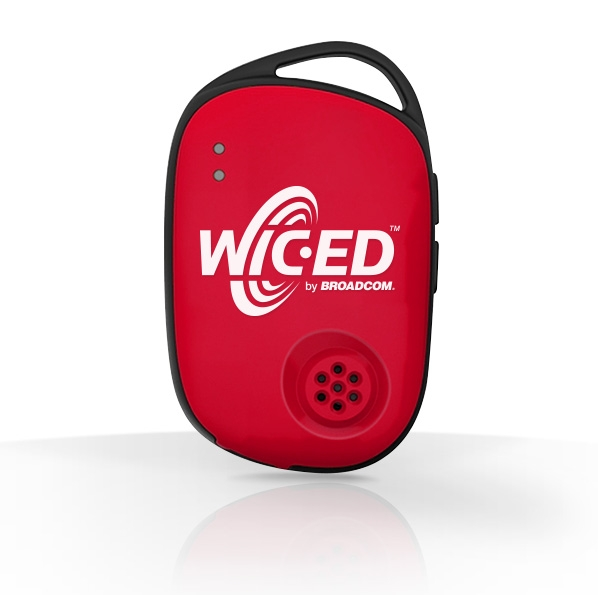
\includegraphics[scale=0.5]{WICED_SENSE.jpg}
	\end{figure}
	

    \begin{itemize}
    \item WICED Sense is a BLE device manufactured by Broadcom* which can provide wireless connectivity to wide range of embedded applications.
    \item The WICED Sense TAG is made up of the BCM20737S Bluetooth Low Energy SoC and five ST Microelectronics sensors: gyroscope, accelerometer, magnetometer , pressure, humidity and temperature. The BCM20737S connects directly to the sensors without the need for an external microprocessor.(* 5 July,2016 onwards Broadcoms IoT business is acquired by Cypress.)
    \item ST Microelectronics Devices used in the WICED Smart Kit:
    \begin{itemize}
    \item Gyroscope (L3GD20)
    \item Accelerometer (LIS3DSH)
    \item Magnetometer (LSM303D)
    \item Pressure sensor (LPS25H)
    \item Humidity and Temperature sensor (HTS221)
    \end{itemize}
	\end{itemize}
	
  \href{http://www.mouser.in/new/broadcom/broadcom-bcm9wiced-sense/}{Wiced Sense Vendor Link }\\
  \href{https://github.com/eYSIP-2016/Wiced-Sense/blob/master/Documentation/Introduction%20to%20Wiced%20Sense/Introduction_to_Wiced_Sense.pdf}{Wiced Sense Introduction }
  
  \newpage
  
  \begin{figure}[h]
    \centering
	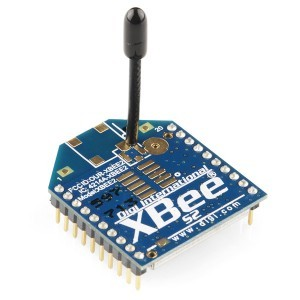
\includegraphics[scale=0.4]{zigbee.jpg}
	\end{figure}
  \item Zigbee Module
  
  \begin{itemize}
    \item ZigBee is an IEEE 802.15.4-based specification for a suite of high-level communication protocols used to create personal area networks with small, low-power digital radios.

    \item The technology defined by the ZigBee specification is intended to be simpler and less expensive than other wireless personal area networks (WPANs). Applications include wireless light switches, traffic management systems, and other consumer and industrial equipment that requires short-range low-rate wireless data transfer.

    \item Its low power consumption limits transmission distances to 10–100 meters line-of-sight. ZigBee is typically used in low data rate applications that require long battery life and secure networking (ZigBee networks are secured by 128 bit symmetric encryption keys.)
    \end{itemize}
  
  \item Firebird V ( Atmega 2560 )
  \begin{figure}[h]
    \centering
	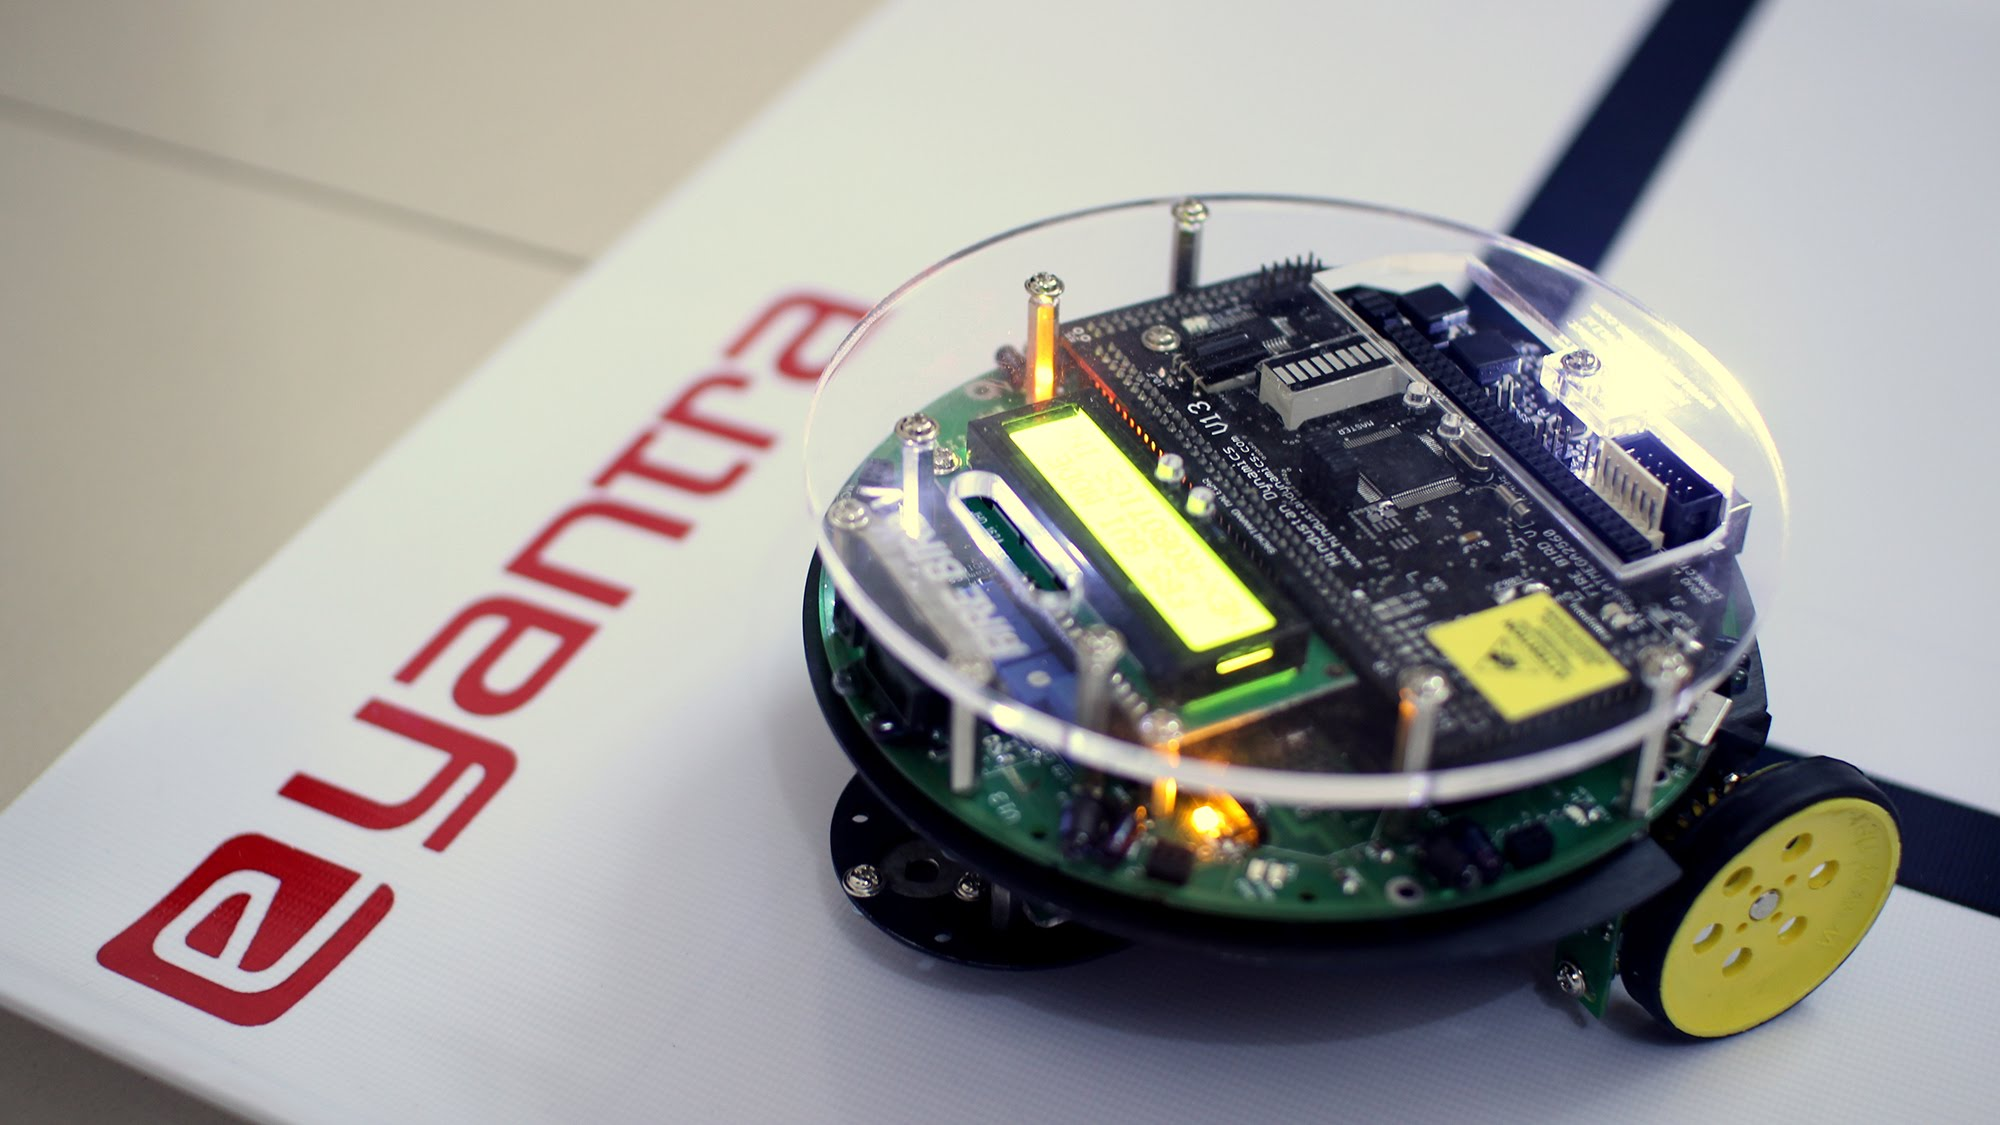
\includegraphics[scale=0.1]{firebird.jpg}
	\end{figure}
  
  
  \newpage
\section{Software Components}
  
  
  \begin{itemize}
  \item Linux Environment 
    \begin{itemize}
     \item Node Js
   
    \begin{figure}[h]
    \centering
	
\includegraphics[scale=0.4]{nodejs.png}
	\end{figure}
   
    \begin{itemize}
    \item Node.js is a platform built on Chrome's JavaScript runtime for easily building fast and scalable network applications. Node.js uses an event-driven, non-blocking I/O model that makes it lightweight and efficient, perfect for data-intensive real-time applications that run across distributed devices.
	\item An important thing to realize is that Node is not a webserver. By itself it doesn't do anything. It doesn't work like Apache. 
    \end{itemize}
  
  \item Cylon Js
  \end{itemize}
    \begin{figure}[h]
    \centering
	
\includegraphics[scale=0.3]{CylonJS.png}
	\end{figure}
    \begin{itemize}
    \item 	Cylon.js is a JavaScript framework for robotics, physical computing, and the Internet of Things. It makes it incredibly easy to command robots and devices.
	\item Cylon.js has an extensible system for connecting to hardware devices. Compatiblity of the hardware can be found at https://cylonjs.com/
	\item Cylon js supports wiced sense. It has support to BLE (Bluetooth Low Energy) devices.
	\end{itemize}
  
  
  \item \href{https://github.com/eYSIP-2016/Wiced-Sense/tree/master/Tutorials/Installation_procedure_in_ubuntu}{Installation Procedure} for the softwares.
  \end{itemize}
  
    \newpage
    \item Windows Environment
    \begin{itemize}
  
  \item Wiced Sense SDK
    \begin{figure}[h]
        \centering
    	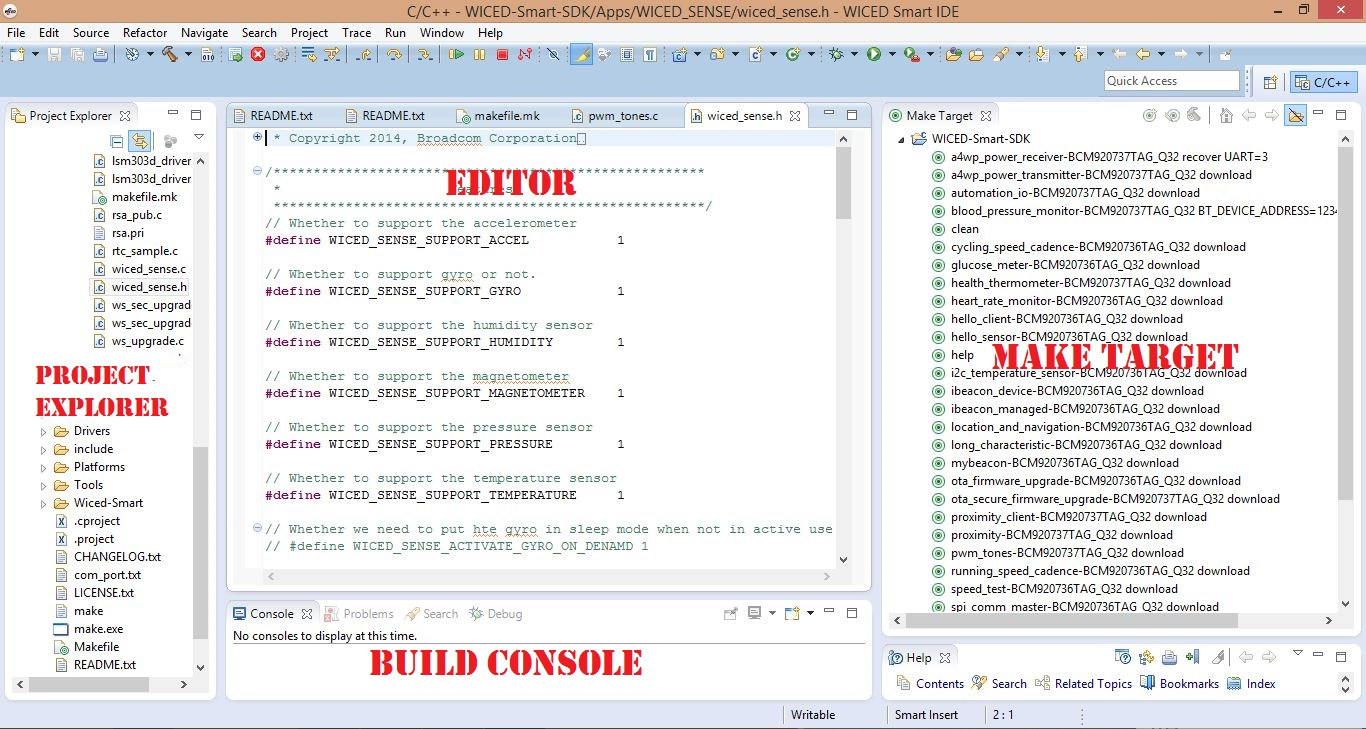
\includegraphics[scale=0.3]{Wiced-sdk.JPG}
	    \end{figure}
	    
	    It is used to program the Wiced Sense Kit.
	\\
   \item Atmel Studio 
            \begin{figure}[h]
        \centering
    	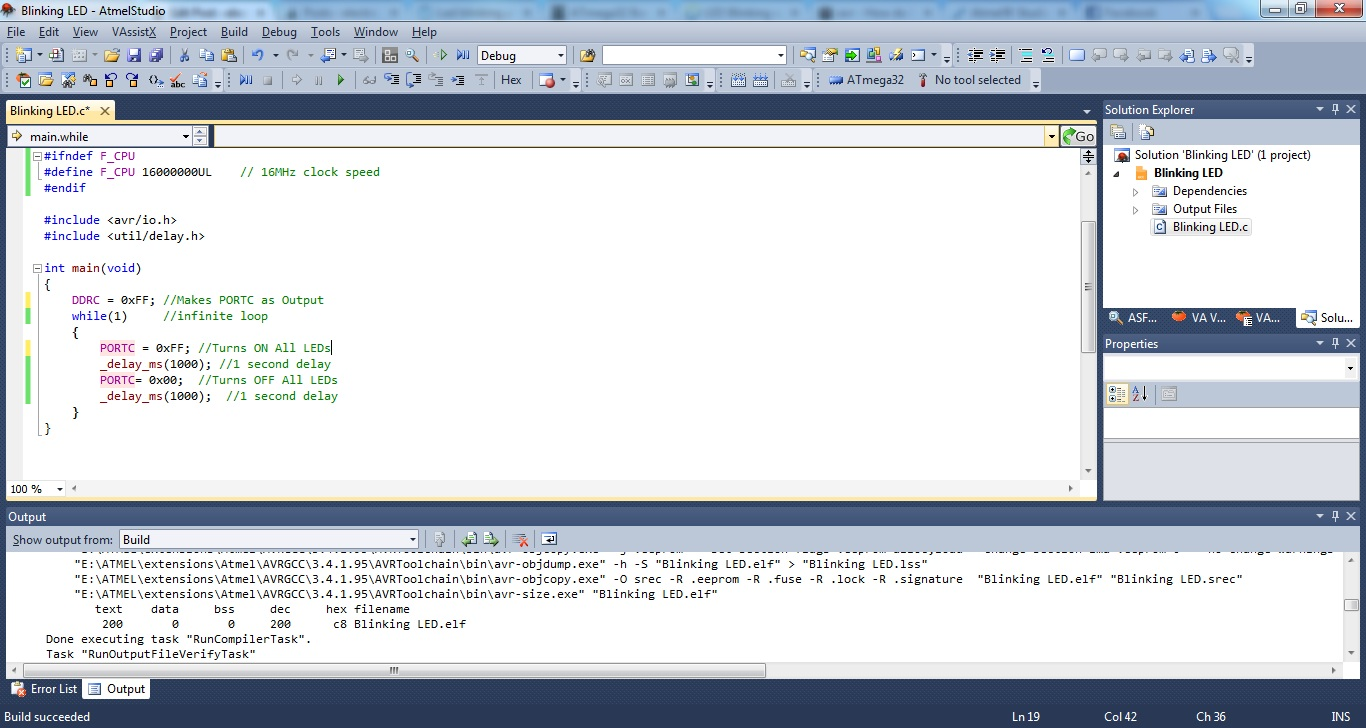
\includegraphics[scale=0.3]{atmel.jpg}
	    \end{figure}
	    
	    It is used to program Firebird V robot.
	    
	    \newpage 
	     \item AVR Bootloader
	     \begin{figure}[h]
        \centering
    	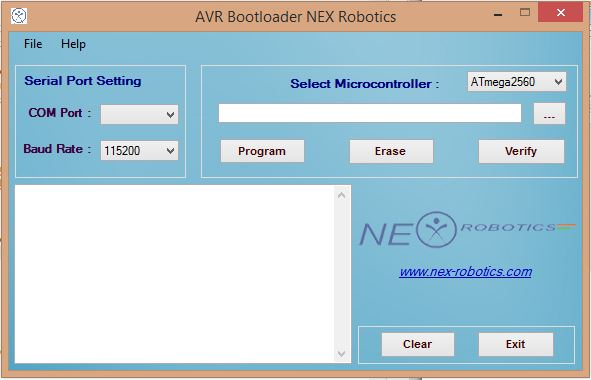
\includegraphics[scale=0.4]{avr.JPG}
	    \end{figure}
  
  It is used to burn code into Firebird V.
  
  \item XCTU
	     \begin{figure}[h]
        \centering
    	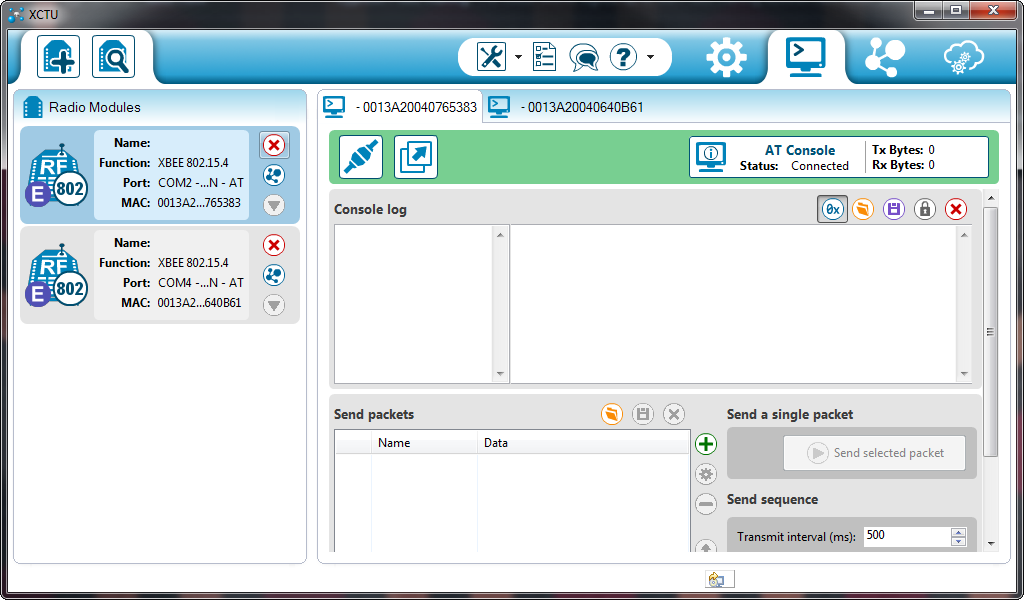
\includegraphics[scale=0.5]{xctu.png}
	    \end{figure}
  
  It is used to configure Zigbee Module.
  
 \end{itemize} 
\end{itemize}

\newpage
\section{Data Flowchart}
  \begin{figure}[h]
        \centering
    	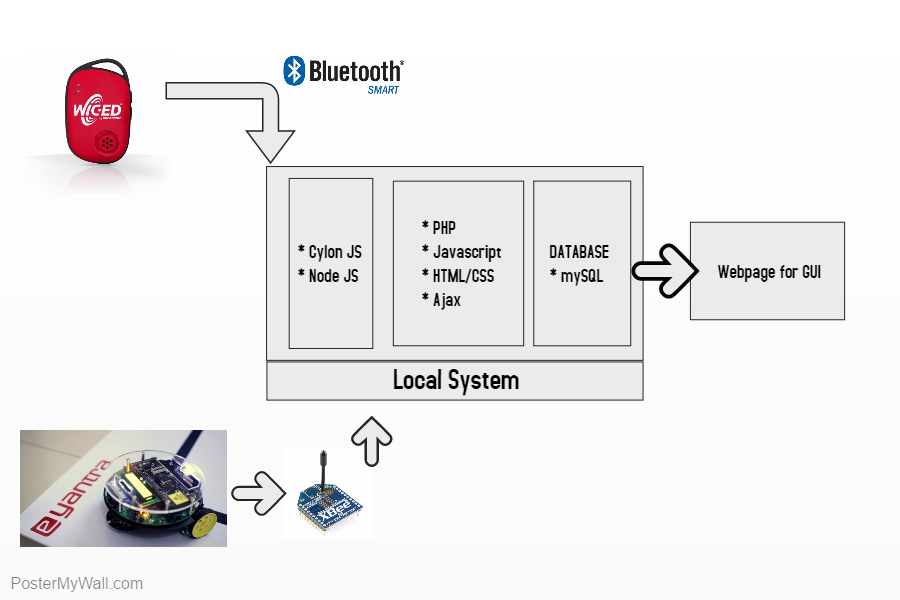
\includegraphics[scale=0.5]{Flowchart.jpg}
	    \end{figure}
\begin{itemize}
  \item The diagram represents the data flow diagram in our project.
  \item Wiced Sense is a BLE (Bluetooth Low Energy) device. It sends the data through Bluetooth to our local system, in our case ubuntu. We need to make sure that our system is BLE compatible.
  \item All the sensor data whose default packet format is explained in \href{https://github.com/eYSIP-2016/Wiced-Sense/blob/master/Documentation/Sensor%20Data%20Format/Sensor_Data_Format.pdf}{Wiced Data Format} is sent to the local system in hex format.

  \item The data is taken into local system with the help of cylon-wiced-sense module. This is the link for cylon-wiced-sense codes.
  \href{https://github.com/eYSIP-2016/Wiced-Sense/blob/master/Codes/Nodejs/wiced-sense.js}{wiced-sense.js}
  \href{https://github.com/eYSIP-2016/Wiced-Sense/blob/master/Codes/Nodejs/driver.js}{driver.js} Its working is explained in codes.
  

  \newpage
  \item Firebird is coded to follow the white line and send the distance travelled by the robot to the local system using zigbee. Distance travelled by the robot is given by the wheel encoders. The link to the code is given \href{https://github.com/eYSIP-2016/Wiced-Sense/tree/master/Codes/FireBird_Codes/Firebird2}{here}
  \item The data of both the wheel encoders are sent.
  \item The node module serialport is used to take the data recieved on local machine through zigbee into cylon code.
  \item Combination of wiced data and encoder data is used for bot mapping which 
  is explained later in the report.
  \item All the data recieved is then parsed and sent to php code using a node module querystring.
  \item It uses POST method to send data via URL to PHP.
  \item The PHP code whose link is provided \href{https://github.com/eYSIP-2016/Wiced-Sense/blob/master/Codes/wiced%20web/controller/test.php}{here} takes the data from URL and updates the tables in the SQL database using SQL query.
    
  \item Now the current webpage calls a PHP page asymmetrically at the server which gets the latest updated data from mySQL database and pass it to webpage via ajax. The link to php code is given \href{https://github.com/eYSIP-2016/Wiced-Sense/blob/master/Codes/wiced%20web/controller/new.php}{here}
  
  \item The data recieved on webpage is used for changing the GUI dynamically. The algorithms are created and the coding of calculations is done in javascript.
  
  \item The webpage for each application is different and is explained further.
\end{itemize}







\newpage
\section{Webpage Description}

\subsection{Sensor GUI page}

\begin{figure}[h]
        \centering
    	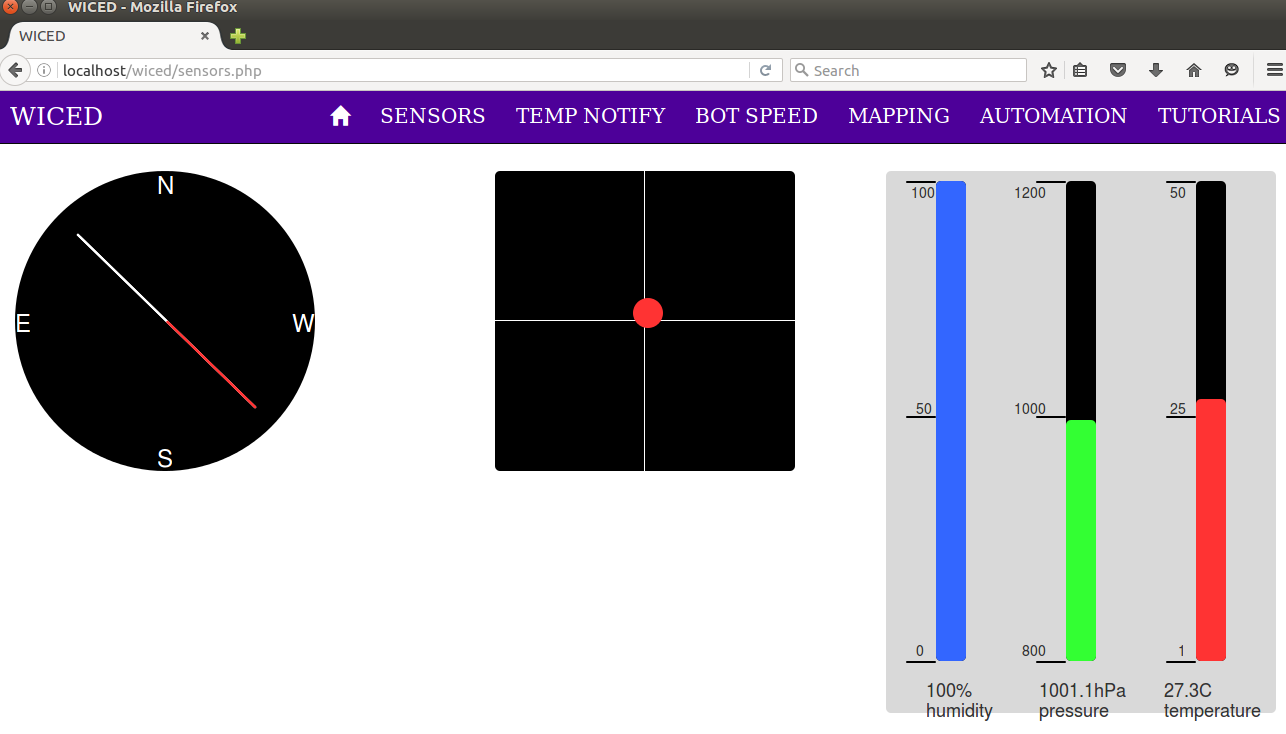
\includegraphics[scale=0.2]{sensor.png}
	    \end{figure}
	    
	    \hspace{5mm}We have made this GUI inorder to display the sensor readings in human understandable form.\\ As seen in the image GUI consists of a compass , whose needle's direction is changed according to rotation of the wiced tag with respect to earth's north pole.
        \\The Bubble level indicated the accelerometer readings. The bubble level shifts according to the acceleration in particular direction.
        \\The 3 bars at the right of the page display the current temperature , pressure and humidity.\\

        \textbf{Code Description}
        
        \begin{itemize}
        \item GUI for this page is made using CSS and HTML.
        \item This page continuously (10ms) makes a request to new.php page at server using an AJAX call.
        \item new.php page extracts all sensor data from mySQL tables using query and returns the extracted data to the sensor page after converting it into JASON format.
        \item This Jason format is parsed and all the sensor data are calculated separately to plot or change the gui dynamically.
        
        \item The link for the code is given \href{https://github.com/eYSIP-2016/Wiced-Sense/blob/master/Codes/wiced%20web/javascript/sensors.js}{here}
        \end{itemize}




\newpage
\subsection{Temperatutre notifier page}



\begin{figure}[h]
        \centering
    	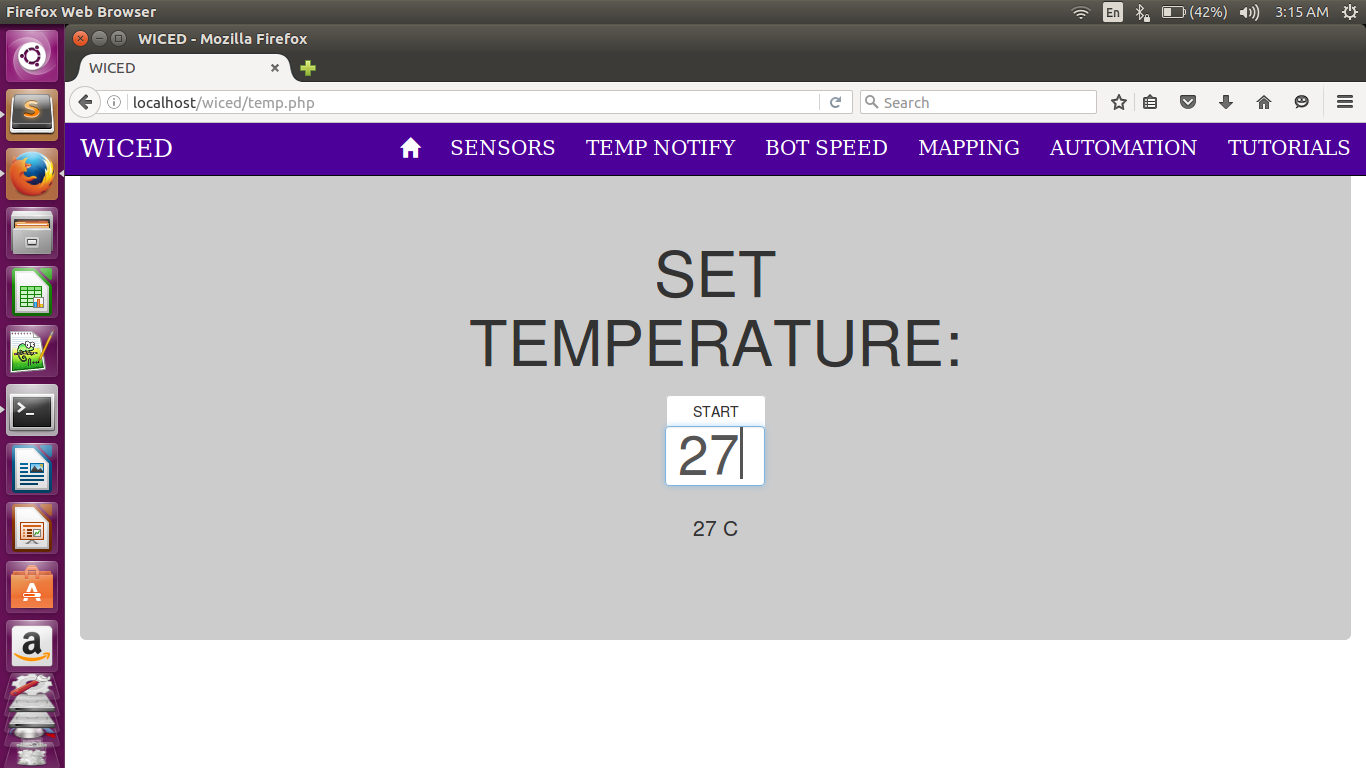
\includegraphics[scale=0.2]{temp12.png}
	    \end{figure}
	    
	    
 This page allows the user to set a particular temperature to trigger a event. The user sets the temperature by entering the temperature in the text box and hits start. Then this value is set as a threshold and a pop up appears if the temperature exceeds the limit.\\

  \textbf{Code Description}
 \begin{itemize}
        \item GUI for this page is made using CSS and HTML.
        \item This page sets the threshold temperature via HTML form and submit it to test.php
        \item test.php updates the threshold temperature value to mySQL database.
        \item This page continuously (10ms) makes a request to new.php page at server using an AJAX call.
        \item new.php page extracts temperature sensor data from mySQL tables using query and returns the extracted data to the temperature page after converting it into JASON format.
        
        \item Jason value of the sensor data is parsed and temp sensor data is calculated and compared with fixed/selected threshold temperature value
        \item As soon as the current temperature goes above fixed temperate, a popup alarm is raised using javascript alert.
        
        \item The link for the code is given \href{https://github.com/eYSIP-2016/Wiced-Sense/blob/master/Codes/wiced%20web/javascript/temp.js}{here}
        \end{itemize}



























\newpage
\subsection{Bot mapping page}

\begin{figure}[h]
        \centering
    	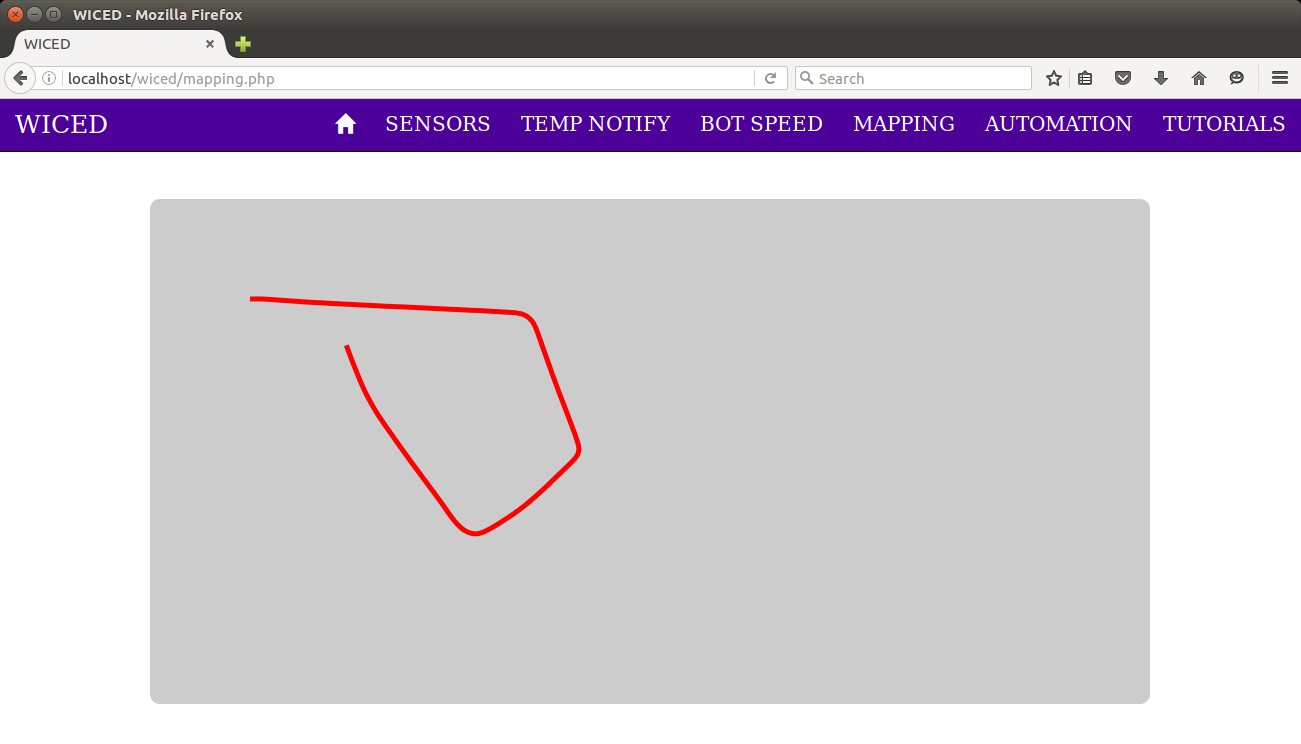
\includegraphics[scale=0.3]{mapping12.png}
	    \end{figure}
	    

This page provides a visualization of the real time movement of the robot. It uses SVG to draw the map. The path of the bot is traced on the screen as the bot proceeds.It uses data from the magnetometer to determine the angle of rotation and the value of encoder to give the distance travelled so as to facilitate path mapping.

 \textbf{Code Description}
        
        \begin{itemize}
        \item GUI for this page is made using CSS and HTML.
        \item This page continuously (10ms) makes a request to new.php page at server using an AJAX call.
        \item new.php page extracts the sensor data of magnetometer and encoder of bot from mySQL tables using query and returns the extracted data to the mapping page after converting it into JASON format.
        \item This Jason format is parsed and all the sensor data are calculated separately to plot or change the gui dynamically.
        \item Magnetometer and Encoder readings are used to achieve bot path mapping using HTML SVG's
        \item The link for the code is given \href{https://github.com/eYSIP-2016/Wiced-Sense/blob/master/Codes/wiced%20web/javascript/mapping.js}{here}
        \end{itemize}














\newpage
\section{Future Work}
\begin{itemize}
\item{Large Scale Purpose}
\begin{itemize}
\item{As the wiced contains accelerometer, gyroscope and magnetometer, it can be used for 3D mapping of an areana.}
\item{The wiced has total 5 sensors, so this tag can be used to create IOT applications}
\end{itemize}
\item{Small Scale purpose}
\begin{itemize}
\item{Wiced can be used as smart tags that can be attached to objects which are likely not to be found while in a hurry eg.keychain}
\item {It can be used to replicate the drawings made on the floor on the computer screen for further processing.}
\end{itemize}
\end{itemize}


\section{Bug report and Challenges}
\begin{itemize}
\item{Bugs}
\begin{enumerate}
    \item{Sometimes their is connection loss between wiced tag and PC (mostly the case of low battery)}
    \item{During mapping sometimes the point deviates from orignal position}
\end{enumerate}
\item{Challenges Faced}
\begin{enumerate}
    \item{Installing all the modules in cylon js and node js.}
    \item{Sending data from cylon code to mySQL database.}
    \item{Path mapping of firebird robot on webpage}
\end{enumerate}
\item{Work Halfdone}
\begin{enumerate}
    \item{Calculating velocity using wiced sense.}
\end{enumerate}
\end{itemize}


\newpage
\begin{thebibliography}{li}

\bibitem{Path design}
SVG Tutorial, {\em SVG path, SVG line, Stroke}  
\href{http://www.w3schools.com/svg/}{Website link}

\bibitem{Data Calculation}
JavaScript Math Reference, {\em math.abs, math.ceil , math.round , math.atan2}  
\href{http://www.w3schools.com/jsref/jsref_obj_math.asp}{Website link}

\bibitem{Node Js}
Node js, {\em querystring, serialport}  
\href{https://nodejs.org/}{Website link}



\end{thebibliography}


\end{document}

